\chapter{Feature Theory}
\label{cp:featuretheory}
\epigraph{Differences which have differentiating value are, as we have seen, more
accessible to perception and to memory than differences which have no value at
all, but on the other hand differences between phonemes—since they lack
particular meanings—strain perception and memory and necessarily require a
great deal of them. We would expect, therefore, that the number of these
primordial and unmotivated values would be relatively small for any given
language.}{Roman Jakobson (1942)}

Speech sounds are continuous signals in the physical world, but somewhere on the communication process they are interpreted by humans as discrete categories. This process of perceiving physical world stimuli into a discrete set of categories is called categorical perception (CP). It might be regarded as a sensory phenomena of percept invariance when experiencing a stimulus that is varied along a continuum.  According to the CP view a phenomenon tend to be perceived in terms of the categories that we have formed. Multiple stimuli are mapped into a single category and there is a sharp change of perception at a certain point in the continuum along which a stimulus may change \citep{liberman1957}. Our perceptions are biased such that differences between objects that belong to different categories are accentuated, and differences between objects that fall into the same category receives little attention. That means, humans have a great ability to perform interclass segregation, but very poor capability to segregate intraclass stimuli. CP has been found in a wide range of stimuli, including the perception of color boundaries \citep{korda1984}, phonemes \citep{liberman1957} and facial expressions \citep{etcoff1992}. In speech, categorical perception suggests that speech perception involves a phonemic encoding step, where the perceptual input is represented in terms of discrete phonemic category labels \cite{liberman1957}. According to \cite{kuhl2000} the encoding process could distort perception stretching distances in regions in which stimuli are equidistant between prototypes (i.e., at phonemic boundaries) and shrinking distances near prototypes.

CP is an important mechanism for processing of naturally occurring stimuli in a continua. It is important to
perceive and respond to objects and events in an environment, in certain situations, it might be critical to the
survival. The ability to ignore redundant sensory variation and cope with the relevant information is necessary
to reduce the processing demands and deal only with relevant information. The variation of stimuli within a category
is much smaller than the variation across different categories. Creating categories and grouping objects is
a task that simplifies further processing.

A good illustration of categorization happens when we observe the colors of a rainbow. Although we though it
is made of a smooth range of light frequencies, we perceive the rainbow as bands with distinct colors.
If we compare the colors in the rainbow we realize it is easier to distinguish two different shades of colors 
when they come from different color boundaries. When they are from the same color boundaries the task
is harder, even if we select shades of colors with the same frequency difference of the previous pair \citep{korda1984}.

The phonemes of a language, as proposed by Saussure, are seen as atomic symbols, indivisible by its nature. The idea of indivisible sound units capable of forming meaningful strings was introduced into the Greek philosophical literature under the name \textit{stoicheia}. ``The sound shape of language and correspondingly its alphabet were viewed as a joint coherent system with a limited number of discrete and interconnected formal units. This concept proved to be so persuasive that Democritus (fragment A6; cf. Diels and Wilpert) and his adherent Lucretius, in searching for an analogy which might confirm their theory of the atomic structure of the physical universe, cited \textit{stoicheia} as the minimal components of speech''\citep{jakobson2002}. One question that rises is whether this belief holds or not in reality. Is it possible to divide and analyze the phonemes using some criteria? Those questions bring along the doubt on what speech sounds are. We know humans can produce many other sounds that are not used in speech, and many sounds, unimaginable to be used as speech sounds in one culture, may turn out to be part of some languages speech sounds inventory. In many languages of southern Africa, sound clicks are speech sounds used as consonants in the language. The click sounds are obstruents articulated with two closures. There are five places of articulation at which they occur: dental, lateral, bilabial, alveolar and palatal. The IPA symbols used for them are, respectively: \textipa{[|]}, \textipa{[||]}, \textipa{[\!o]}, \textipa{[!]} and \textipa{[\textdoublebarpipe]}. Some sounds produced by the vocal tract are known not to be used in any language, like whistles, inhalation or a labiolingual trill\footnote{The sound of blowing a raspberry or making a bronx cheer is the sound made by sticking out the tongue between the lips and blowing to make a sound reminiscent of flatulence.} (a.k.a. ``blowing a raspberry''). Those sounds, in other cultures are just regarded as sounds produced with the voice apparatus, 
but are not used as speech sound at all, although they might be used on a non linguistic communication.
%It is important to note that, although these sounds may not be part of speech sounds repertory, they may still be used in communication. The neutral vowel (schwa, \textipa{[@]}) is not part of the Portuguese speech sounds repertory but it is used in communication, for example, to criticize pejoratively someone's mistake, this vowel is frequently used in Brazil.

The sounds used in speech communication are inserted into a continuous of infinitesimal variations in its qualities. What we label as a specific symbol or another may be understood as segmentation of this continuous in a small finite set of unities that will be used as the symbols to build speech communication. Consider, for example, the vowels \textipa{[e]} and \textipa{[E]}. What is perceived in each culture may be slightly different, the prototypical \textipa{[e]} in one language may be lower than the prototypical \textipa{[e]} in another language, but not low enough to be considered as a \textipa{[E]} by any of those languages. The place where different cultures imposes a threshold to segregate different vowels in a continuous may differ. Those differences among languages may be perceived when someone is learning a foreign language. Even if the same sounds are shared between one's mother tongue and a certain foreign language, the discretization process to create prototypes in each language may not be the same, and some slight noticeable differences may appear, what makes it hard to speak a foreign language with no accent at all. \cite{peterson} show that, although there is a great correlate between vowel categorization by listeners and vowels physical properties (frequency of the first and second formants, in this case), the boarder between them is not sharp. There is a fuzzy transition among all the perceived vowels, and in certain regions it is hard to tell whether the physical observation is of one vowel or another. This is well illustrated in the Figure \ref{fig:vowelsF1F2}.

\begin{figure}[h!]
\centering
\includegraphics[width=0.85\textwidth]{images/vowelsF1F2.png}
\caption{Frequency of second formant \textit{versus} frequency of first formant for vowels spoken by men and children, which were classified unanimously by all listeners. (Figure reproduced from \citep{peterson})}
\label{fig:vowelsF1F2}
\end{figure}  

What is important, under the concern of phonology, is what are speech sound differences capable of being differentiated in a language and eliciting different meaning. Answering this question is the same as answering the question `what is a possible phoneme?'. The answer to these questions is not trivial, and it involves not only the way humans perceive speech under a certain culture, but also how human perceive the world. Some cognitive aspects of perception are universal. The very fact of perceiving the continuous world as a discrete set of types instead of tokens\footnote{The distinction between \textit{types} and \textit{tokens} is an ontological one, it is the difference between a general sort of things and a concrete instance of this sort. We say then that \textit{tokens} are instances of a \textit{type}.} is a commonplace in speech perception as well as in color perception. If we consider the way humans perceive a rainbow, the categorization into seven bands of colors is an artifact of human perception, a rainbow is in fact a continuous spectrum of colors. That seems like the magical number seven playing its role in human categorization. According to the Miller's Law \citep{miller1956}, the number of objects, on average, that a human can hold in working memory is $7 \pm 2$.

The way how speech sounds are perceived is rather subjective. One study performed by \cite{laboissiere2010} shows how the phonemic distinction between \textipa{/e/} and \textipa{/E/} takes place for German speakers. A series of stimuli was presented to the subjects of this experiment. The stimulus were a computer generated continuous transition from \textipa{[e]} to \textipa{[E]} that were presented in the context of the minimal pairs in German \textit{fell} (\textipa{[fEl]}) vs. \textit{fehl} (\textipa{[fe:l]}). They were asked to indicate when the transition from one word into another happened. This experiment shows that in the enormous continuum between one prototypical phonemic realization and another, all the instances found are perceived either as one prototype or another, in this wide space there is place only for two possible categorizations.

It is important to note that the contrast shown by \cite{laboissiere2010} is between two vowels of different quality and duration: \textipa{[e:]} and \textipa{[E]}. In German, the short vowels \textipa{[i, y, u, e, \o, o]} occur only in unstressed syllables of words borrowed from other languages. They are usually considered complementary allophones together with their long counterparts which cannot occur in unstressed syllables. In this situation, it is difficult to say what is the share of contribution of tenseness (tense vs. lax) and length (short vs. long) contrasts into the categorization process.

``The striking thing about phonology is that the infinite phonetic variety in the utterances of any language can be reduced to a small inventory of contrastive units or phonemes''\citep{hualde2004}. This inventory is created through a linguist investigative analysis in order to state the building blocks that will assemble one language. This analysis process is many times controversial, it is difficult to establish a consensual phonemic contrast. Even at the phonetic level, it is not easy to choose the right representation, since speech utterances may have different realizations. \cite{hualde2004} shows an example in Basque where the word \textit{mollako} is pronounced in many ways, regarding the sound of the consonant \textit{k} that is usually voiceless but sometimes voiced and other times partially voiced. That brings a question on which phonetic transcription to choose. This problem is also not solved at the phonemic level because the phonemic status of some palatal consonants in Basque is controversial. The word \textit{mollako} could be then transcribed in two ways: \textipa{/moLako/} or \textipa{/moilako/}. ``In the relevant Basque dialects \textipa{/l/} palatalizes after \textipa{/i/} and palatal glides are absorbed by a following palatal lateral, so that both phonemic inputs would result in the same output''\citep{hualde2004}. Just as in other domains, a categorization process may involve different levels. \cite{ladd} shows that exists, in French and Italian, a special link between the mid vowels \textipa{/e/} and \textipa{/E/} that is not found between \textipa{/e/} and \textipa{/i/}, as previously remarked by \cite{trubetzkoy}. Category boundaries may be fuzzy and in certain aspects multi-level, allowing overlaps between them. As observed by \cite{hualde2004}, the questionable phonemes in Spanish (\textipa{j} and \textipa{J}) followed by an \textipa{[a]} may be mistaken by the hiatus sequence \textipa{ia}. The overlap shown by this example is dependent of the Spanish dialect, what shows that the categorization process may be done in different ways. As previously remarked by \cite{saussure}, ``En matière de langue on s’est toujours contenté d’opérer sur des unités mal définies''\footnote{In language's matter it has always been sufficient to operate on ill-defined units.}.

The distinctive feature theory rises as a way to characterize the speech sounds in term of features and use those features to derive phonological explanation of how languages work. It is impractical to establish phonological rules based on physical descriptions of speech sounds. For example, a rule that says that a vowel sound suffer a increase in its first formant frequencies by 205Hz and by 430Hz in its second formant frequency when preceded by another vowel whose first formant frequency is lower than 410Hz, is so much an inefficient way of describing a phonological processes. It is much simpler to describe it in another fashion, in a qualitative form, because we know that the relationships, not the absolute values of physical properties of speech sounds, are important. It is much easier to say that a near-front vowel is transformed into a front vowel when preceded by a front vowel. This qualitative rule is quite simpler and may be used to describe the same phonological rule that is slightly different in distinct languages.

The properties used to describe speech sounds in the distinctive feature theory are general and abstract, that means, their behavior is fuzzy. The theory proposes the existence of a small finite set of features that may be used to analyze speech sounds, in such way that the description of each speech sound in terms of these features is unique. The analysis into distinctive features is a unambiguous process to associate speech sounds into arrays of features that describe these sounds. The classical statement of distinctive features was brought by \citet{chomsky1968a}.
 
The major class features, proposed by \citet{chomsky1968a} are: sonorant, vocalic (syllabic) and consonantal. Those major features provide a rough initial grouping of speech sounds into functional types that includes the consonant/vowel distinction. The sonorant sounds are those in which the vocal tract configuration makes spontaneous voicing possible. In syllabic sounds the constriction does not exceed that of high vowels, and spontaneous voicing is possible. They form a syllable peak and stress may be then applied. The consonantal sounds are those produced with a major obstruction in the mid-sagittal region of the vocal tract.

The set of distinctive features proposed by \citet{chomsky1968a} was afterwards modified by other researchers according to their convenience to better analyze a certain language. Some commonly used features are: consonantal, syllabic, sonorant, continuous, delayed release, nasal, lateral, anterior, coronal, high, back, rounded, low, voiced, tense, strident, ATR (advanced tongue root). The meaning of each feature is described bellow:
\begin{description}
\item[syllabic / non-syllabic] : The syllabic feature characterizes sounds which have a sonority peak within, and we say they constitute a syllable peak. The feature [$+$syllabic] refers to vowels and syllabic consonants. Contrastive examples of syllabic consonants in English are:
\begin{center}
\begin{tabular}{lcl}
syllabic     & \hspace{1cm} & non-syllabic \\
coddling \textipa{[k6d\s{l}IN]} & & codling \textipa{[k6dlIN]} \\
Hungary \textipa{[h2Ng\s{r}i]} & & hungry \textipa{[h2Ngri]} \\
\end{tabular}
\end{center}

\item[consonantal / non-consonantal] : Consonantal sounds are produced with vocal tract constriction, a radical obstruction in the mid-sagital region. Non-consonantal sounds are produced without such an obstruction.

\item[sonorant / obstruent] : ``Sonorants are sounds produced with a vocal tract cavity configuration in which spontaneous voicing is possible'' \citep{chomsky1968a} due to the air pressure on both sides of any constriction to be approximately equal to the air pressure outside the mouth. Obstruent sounds are characterized by a significantly greater air pressure behind the constriction. [$+$sonorant] refers to vowels and approximants (glides and semi-vowels); [$-$sonorant] refers to stops, fricatives and affricates.

\item[coronal / non-coronal] : ``Coronal sounds are produced by raising the tongue blade toward the teeth or the hard palate; noncoronal sounds are produced without such a gesture'' \citep{chomsky1968a}. Some authors argue that this feature applies only to consonants; others argue it may apply to front vowels as well. [$+$coronal] refers to dentals (not including labio-dentals) alveolars, post-alveolars, palato-alveolars, palatals. [$-$coronal] refers to labials, velars, uvulars, pharyngeals.

\item[anterior / posterior] : ``Anterior sounds are produced with a primary constriction at or in front of the alveolar ridge. Posterior sounds are produced with a primary constriction behind the alveolar ridge'' \citep{chomsky1968a}. This feature distinguishes coronal sounds produced in front of the alveolar ridge from those produced behind it. [$+$anterior] refers to labials, dentals and alveolars. [$-$anterior] refers to post-alveolars, palato-alveolars, retroflex, palatals, velars, uvulars, pharyngeals.

\item[labial / non-labial] : Labial sounds are those where there is rounding or constriction at the lips,  one or both lips are the active articulator. [$+$labial] refers to labial and labialised consonants and to rounded vowels

\item[distributed / non-distributed] : ``Distributed sounds are produced with a constriction that extends to a considerable distance along the midsaggital axis of the oral tract; nondistributed sounds are produced with a constriction that extends for only a short distance in this direction'' \citep{chomsky1968a}. Apical from laminal and retroflex from non-retroflex consonants are then distinguished by this feature.
%[$+$distributed] refers to sounds produced with the blade or front of the tongue, or bilabial sounds. [$-$distributed] refers to sounds produced with the tip of the tongue.

\item[high / non-high] : ``High sounds are produced by raising the body of the tongue toward the palate; nonhigh sounds are produced without such a gesture'' \citep{chomsky1968a}. [$+$high] refers to palatals, velars, palatalised consonants, velarised consonants, high vowels, semi-vowels.

\item[mid / non-mid] : some authors add this feature to deal with vowel systems with four contrastive levels of height. Mid sounds are produced with tongue height approximately half way between high and low sounds.

\item[low / non-low] : ``Low sounds are produced by drawing the body of the tongue down away from the roof of the mouth; nonlow sounds are produced without such a gesture'' \citep{chomsky1968a}. [$+$low] refers to low vowels, pharyngeal consonants, pharyngealised consonants.

\item[back / non-back] : ``Back sounds are produced with the tongue body relatively retracted; nonback or front sounds are produced with the tongue body relatively advanced'' \citep{chomsky1968a}. [$+$back] refers to velars, uvulars, pharyngeals, velarised consonants, pharyngealised consonants, central vowels, central semi-vowels, back vowels, back semi-vowels.

\item[front / non-front] : this feature is added to distinct the central vowel, which is [$-$back] and [$-$front].

\item[continuant / stop] : ``Continuants are formed with a vocal tract configuration allowing the airstream to flow through the midsaggital region of the oral tract: stops are produced with a sustained occlusion in this region'' \citep{chomsky1968a}. [$+$continuant] refers to vowels, approximants, fricatives. [$-$continuant] refers to nasal stops, oral stops. Some authors also make a distinction between [continuant acoustic] and [continuant articulatory]. The English nasals \textipa{[m,n,N]} are then [$+$continuant acoustic] but [$-$continuant articulatory].

\item[lateral / central] : ``Lateral sounds, the most familiar of which is \textipa{[l]}, are produced with the tongue placed in such a way as to prevent the airstream from flowing outward through the centre of the mouth, while allowing it to pass over one or both sides of the tongue; central sounds do not invoke such a constriction'' \citep{chomsky1968a}. [$+$lateral] refers to lateral approximants, lateral fricatives, lateral clicks.

\item[nasal / oral] : ``Nasal sounds are produced by lowering the velum and allowing the air to pass outward through the nose; oral sounds are produced with the velum raised to prevent the passage of air through the nose'' \citep{chomsky1968a}. [$+$nasal] refers to nasal stops, nasalised consonants, nasalised vowels and  less-common pre-nasalized stops, nasal glides, nasal fricatives, and nasal trills.

\item[tense / lax] : This feature applies to vowel characterization, the traditional definition is that tense vowels present a greater constriction than lax vowels. In some languages, the tense/lax distinction is also made between long/short vowels. A more general definition, states that the tense/lax distinction is related to some kind of strong/weak contrast. In some languages, this distinction is made between more peripheral vowels (closer to the four corners of the vowel quadrilateral) and less peripheral vowels (more centered and/or more mid vowels).

\item[sibilant / non-sibilant] : Sibilants are a type of fricative or affricate consonants, resulted from the production of a jet of air through a narrow channel in the vocal tract towards the sharp edge of the teeth. They have then large amounts of acoustic energy at high frequencies, and sound then louder than their non-sibilant counterparts. [$+$sibilant] refer to the following sounds: \textipa{[s,S,z,Z]}.

\item[spread glottis / non-spread glottis] : ``Spread or aspirated sounds are produced with the vocal cords drawn apart producing a nonperiodic (noise) component in the acoustic signal; nonspread or unaspirated sounds are produced without this gesture'' \citep{chomsky1968a}. This feature is used to indicate the aspiration of a segment. [$+$spread glottis] refers to aspirated consonants, breathy voiced or murmured consonants, voiceless vowels, voiceless approximants.

\item[constricted glottis / non-constricted glottis] : ``Constricted or glottalized sounds are produced with the vocal cords drawn together, preventing normal vocal cord vibration; nonconstricted (nonglottalized) sounds are produced without such a gesture'' \citep{chomsky1968a}. [$+$constricted glottis] refers to ejectives, implosives, glottalized or laryngealised consonants, glottalized or laryngealised vowels.

\item[voiced / voiceless] : ``Voiced sounds are produced with a laryngeal configuration permitting periodic vibration of the vocal cords; voiceless sounds lack such periodic vibration'' \citep{chomsky1968a}. When the segment is characterized as [$+$voiced], the vibration of the vocal folds occurs concomitantly with its articulation.

\end{description}


Although those features are used to characterize speech sounds, in some situations it makes no sense to use some attributes to some sounds. To characterize vowels as [$+$strident] or [$-$strident], [$+$lateral] or [$-$lateral] is something that does not concern the nature of vowels.
%, it would be like characterize a pencil as loud or not, since this attribute does not characterize a pencil, although you make use it to create loud noise. 
In the same way, the height of a vowel may be characterized by the features high and low. High vowels are [$+$high] and [$-$low], low vowels are [$+$low] and [$-$high]. No vowel can be simultaneously [$+$high] and [$+$low]; but mid vowels are said to be [$-$high] and [$-$low] at the same time.

Some feature combinations are considered impossible. The combination [$-$sonorant, $-$consonantal], for example, is said as a physical impossibility since [$-$sonorant] segments would require a major obstruction in the vocal tract, on the other hand, [$-$consonantal] says that the obstruction cannot be in the oral cavity. The only conclusion would be to require a constriction of the nasal passages, but nostrils are not sufficiently constrictable, leading to a physical incongruence \citep{odden2005}. Another matter that is discussed as an impossibility is whether there are syllabic obstruents segments, i.e. \textipa{[\s{s}]}, \textipa{[\s{k}]}. It has been claimed  to exist in certain dialects of Berber\footnote{The Berber group of languages is formed by indigenous languages of North Africa west of the Nile. They are spoken mainly in Morocco and Algeria.} \citep{odden2005}, but it is still a controversial matter.

The most important contribution to phonology from the distinctive feature theory is that a set of segments may be analyzed into some features and it is possible to identify classes of segments in rules, creating the notion of \textit{natural class}, as a set of sounds that has certain phonetic features in common and is affected in the same way in the same environment. Natural classes can be defined by the combination of some features. For example, [$+$consonantal, $-$syllabic], referring to a set of segments which are simultaneously [$+$consonantal] and [$-$syllabic]. In order to create a natural class,  made of two or more segments, it is necessary that the number of features used to specify this class to be less then the number of features to specify each element inside this class. The three major class features may be used to define together five maximally differentiated classes, as shown in the table bellow:

\begin{table}[h!]
\centering
\begin{tabular}{llllll}
 			& \textipa{a, i, u} & \textipa{\s{r}, \s{l}, \s{m}} & \textipa{y, w, h, P} & \textipa{r, l, m} & \textipa{s, z, p, b} \\
 syllabic		& $+$ & $+$ & $-$ & $-$ & $-$ \\
 sonorant		& $+$ & $+$ & $+$ & $+$ & $-$ \\
 consonantal	& $-$ & $+$ & $-$ & $+$ & $+$ 
\end{tabular}
\end{table}
Further classes are definable by omitting specifications of one or more of these features: for example, the class [$-$syllabic, $+$sonorant] includes \{\textipa{y, w, h, P, r, l, m}\}. As defined by \cite{flemming2005}, ``natural classes derive from the nature of the set of markedness constraints. For example, sounds can pattern together as a natural class if they violate markedness constraints in the same environment, so given constraints *XA and *XB, A and B can form a natural class''. To the set of speech sounds that form a natural class, it may be given a simpler phonetic categorization. Speech sounds that are in a natural class, usually undergo together in a phonological process. ``Sounds do not constitute a natural class just because they share feature specifications, the class must contain all the sounds that have those feature specifications''\citep{flemming2005}.

According to the theory of phonological features, phonemes are characterized according to a finite set of features. Those features are called distinctive features for there are no two phonemes that share the same features. If they do so, they are the same phoneme. The features are grouped into categories: major class features, laryngeal features, manner features and place features. Features are usually specified in a binary manner, by assigning a positive value [+] to denote the presence of a feature and a negative value [-] to indicates its absence. 

The distinctive feature table proposed for the Brazilian Portuguese is represented in the Figure \ref{fig:distinctivefeaturetable}. In this representation we assign the color white to the features that we would assign `$+$' and black to the features we would assign `$-$'. With this form of representation it is easier to realize which features are shared by some speech sounds.

\begin{figure}[h!]
\centering
\includegraphics[width=0.85\textwidth]{images/distinctivefeature_PT_matrix.pdf}
\caption{Distinctive feature table for the Brazilian Portuguese.}
\label{fig:distinctivefeaturetable}
\end{figure}

Using this representation of speech sounds into an array of sound features, we may define a distance measure of two segments as the number of features not shared between them (that dissimilarity definition resembles the natural class definition of \cite{flemming2005}). Using this definition of distance we conclude that the distance between the segments \textipa{[k]} and \textipa{[h]} is only one, since the only feature they do not share is [continuous], \textipa{[k]} is described as [$-$continuous] and \textipa{[h]} as [$+$continuous]. This proposed distance may then be used to create a dissimilarity matrix among all speech sounds in the language repertory. The result of this procedure is shown in Figure \ref{fig:dissimilaritymatrix}, where the result is normalized so that the maximum distance found is one and the minimum distance is zero. Analyzing this image, it is easy to recognize two big groups: the vowels and the consonants. It is also easy to recognize visually some other groups, as the group of plosives, the group of fricatives, and the group of nasals.

\begin{figure}[h!]
\centering
\includegraphics[width=0.85\textwidth]{images/dissimilarity_PT_matrix.pdf}
\caption{Dissimilarity matrix for the speech sounds in Brazilian Portuguese.}
\label{fig:dissimilaritymatrix}
\end{figure}

With such a matrix of dissimilarities at hand, we might perform the multidimensional scaling (MDS) of the data. The idea of MDS was first introduced by \citet{young} and it consists of finding a representation of objects in a vector space such that the distance between those representations is in accordance with the dissimilarities presented by the input matrix. 
``Multidimensional scaling, then, refers to a class of techniques. These techniques use proximities among any kind of objects as input. A proximity is a number which indicates how similar or how different two objects are, or are perceived to be, or any measure of this kind. The chief output is a spatial representation, consisting of a geometric configuration of points, as on a map. Each point in the configuration corresponds to one of the objects. This configuration reflects the `hidden structure' in the data, and often makes the data much easier to comprehend'' \citep{kruskal}.

It is important then to choose a suitable metric which leads to a meaningful description of a data space, for wrong descriptions of facts may lead to false results and wrong interpretations. The distinctive feature theory provides a way of characterizing speech sounds based on articulatory, acoustical and perceptual attributes \citep{chomsky1968a}. In this theory, there is a unique representation of each speech sound based on presence or absence of features. This paper uses the theory of distinctive features to create a measure of dissimilarity: a distance measure between two segments defined as the number of features that they do not share.


The input for an MDS method is a dissimilarity (or similarity) matrix $\Delta$:
\begin{equation}
  	\mathbf{\Delta} = 
\left( \begin{array}{cccc}
\delta_{1,1} & \delta_{1,2} & \ldots & \delta_{1,N} \\
\delta_{2,1} & \delta_{2,2} & \ldots & \delta_{2,N} \\
\vdots       & \vdots       & \ddots & \vdots       \\
\delta_{N,1} & \delta_{N,2} & \ldots & \delta_{N,N} \\
\end{array} \right) \textmd{ .}
\end{equation}
  
The dissimilarity (distance) or data value connecting object $i$ with object $j$ is represented by $\delta_{i,j}$.\footnote{In many situations there may be no effective difference in meaning between $\delta_{i,j}$ and $\delta_{j,i}$, and there may be no meaning at all for $\delta_{i,i}$, so that the data values may not form an entire matrix, but only part of one.}

The output of an MDS method is a set of $N$ R-dimensional vectors representing the objects (or stimulus) subjected to the current study:
  
  \begin{eqnarray}
  \mathbf{x_1} &=& \left( x_{1,1}, \ldots, x_{1,R} \right)^T \nonumber \\
  \mathbf{x_2} &=& \left( x_{2,1}, \ldots, x_{2,R} \right)^T \nonumber \\
   &\vdots&  \\
  \mathbf{x_N} &=& \left( x_{N,1}, \ldots, x_{N,R} \right)^T \nonumber
  \end{eqnarray}

To calculate the MDS, we should start by calculating the dissimilarity matrix $\mathbf{D}$ (where, in this case, $\mathbf{D} \approx \mathbf{\Delta}$) of distance between samples of our database. We build then a matrix $\mathbf{A}$ such that: 
\begin{equation}
[\mathbf{A}]_{i,j}=a_{i,j}=-\frac{1}{2}d_{i,j}^2 \textmd{ .}
\end{equation}
A matrix 
\begin{equation}
\mathbf{B}=\mathbf{HAH}
\end{equation}
is calculated, where $\mathbf{H}$ is given by 
\begin{equation}
\mathbf{H} = \mathbf{I} - N^{-1}\mathbf{1}\mathbf{1}^T \textmd{ ,}
\end{equation}
which is positive-semidefinite by construction. 
The matrix $\mathbf{I}$ used is the $N \times N$ identity matrix, and $\mathbf{1}$ is an $N$ dimensional all-ones vector.

The matrix $\mathbf{B}$ is usually a positive-semidefinite matrix (if not, we may add a small constant and make it positive-semidefinite), so that singular value decomposition (SVD) applies: 
\begin{equation}
\mathbf{B} = \mathbf{V} \mathbf{\Lambda} \mathbf{V}^T \textmd{ .} 
\end{equation}
$\mathbf{B}$ is a matrix of rank $p$, then $N-p$ eigenvalues of $\mathbf{B}$ are null and we have
\begin{equation}
\mathbf{B} = \mathbf{V_1} \mathbf{\Lambda_1} \mathbf{V_1}^T \textmd{ ,}
\end{equation}
where $\mathbf{\Lambda_1}=diag(\lambda_1,\ldots,\lambda_p)$ and $\mathbf{V_1} = [v_1,\ldots,v_p]$. As $\mathbf{B}=\mathbf{X} \mathbf{X}^T$, $\mathbf{X}$ is given by 
\begin{equation}
\mathbf{X} = \mathbf{V_1} \sqrt{\mathbf{\Lambda_1}} \textmd{ ,} 
\end{equation}
and we have then calculated the matrix $\mathbf{X}$, which is the representation of the original data in a new vector space where each dimension is a principal component.

Using the dissimilarity matrix created and explained above, an MDS procedure is performed and a representation in two dimensions is shown in figures \ref{fig:mds2Dvowels} and \ref{fig:mds2Dconsonants}. The first plot, represents the vowels of Brazilian Portuguese in a two dimensional space. It is important to note that this 2D plot represents 65\% of the data variance, meaning that more dimensions would be required to take into account all the information of the data. Anyway, analyzing the result, we can easily recognize the dimensions used in the usual vowel diagram (shown in Figure \ref{fig:IPA_Vowels}) where the main distinction is made in terms of \textit{high} and \textit{low}, and \textit{back} and \textit{front}). The dimensions of the MDS representation are in fact a combination of the features \textit{high-low}, and \textit{back-front}. The same sort of analysis may be performed on the MDS representation for the consonants. It is shown in Figure \ref{fig:mds_consonant_PT_class}.

\begin{figure}[h!]
\centering
\includegraphics[width=0.85\textwidth]{images/mds_vowelsPT.pdf}
\caption{2D MDS result for the vowels of Brazilian Portuguese.}
\label{fig:mds2Dvowels}
\end{figure}


\begin{figure}[h!]
\centering
\includegraphics[width=0.85\textwidth]{images/mds_consonantsPT.pdf}
\caption{2D MDS result for the consonants of Brazilian Portuguese.}
\label{fig:mds2Dconsonants}
\end{figure}

\begin{figure}[h!]
\centering
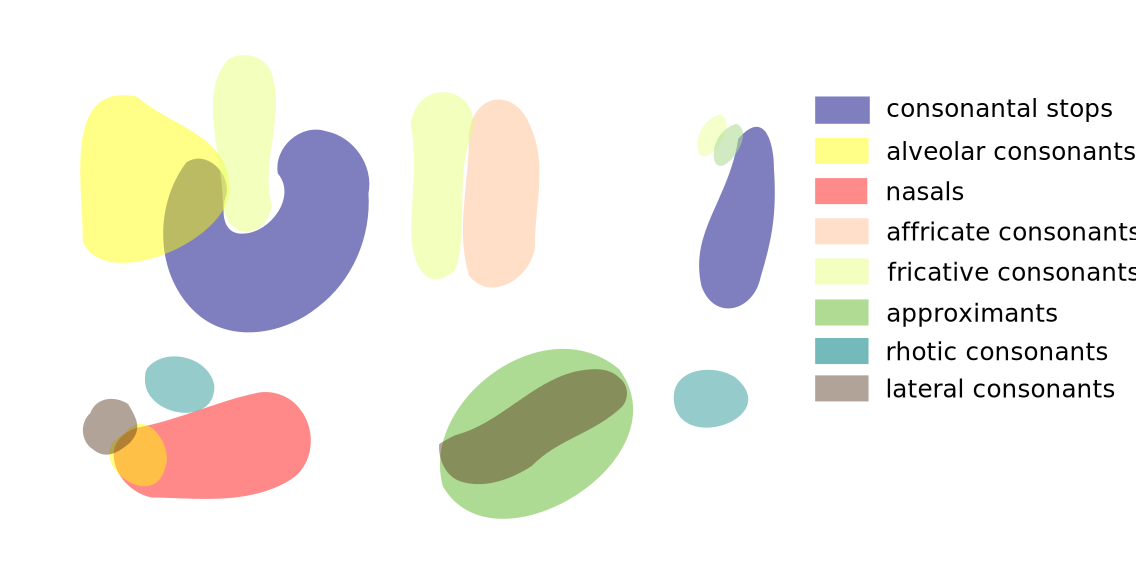
\includegraphics[width=0.95\textwidth]{images/mds_consonant_PT_class.png}
\caption{2D MDS result for the consonants of Brazilian Portuguese.}
\label{fig:mds_consonant_PT_class}
\end{figure}

\begin{figure}[h!]
\centering

\includegraphics[width=0.55\textwidth]{images/IPA_Vowels.pdf}
\caption{Vowel Diagram from the IPA table.}
\label{fig:IPA_Vowels}
\end{figure}

Considering one more dimension, we are capable of creating a representation in three dimensions where now we have 61\% of the data variance explained by this plot. With this new plot it is possible to see a better separation of some speech sounds, the fricative and the plosive sounds are now represented further apart compared to the first representation in two dimensions. 

\begin{figure}[h!]
\centering
\includegraphics[width=0.85\textwidth]{images/mds_consonantsPT_3D.pdf}
\caption{3D MDS result for the consonants of Brazilian Portuguese}
\label{fig:mds3Dconsonants}
\end{figure}

Figures \ref{fig:dissimilaritymatrixM2}, \ref{fig:mds2DvowelsM2}, \ref{fig:mds2DconsonantsM2}, \ref{fig:mds3DconsonantsM2}, are analogous to figures \ref{fig:dissimilaritymatrix}, \ref{fig:mds2Dvowels}, \ref{fig:mds2Dconsonants}, \ref{fig:mds3Dconsonants}, but now the distance metric used is another one. In this new metric we add null if two speech sounds share a feature with a `$+$' attribute; if both share a `$-$' we add $1/3$ to the distance measure, because a `$-$' attribute may be used by something to what this attribute does not make sense; and we add $2/3$ to the other possible situations ([`$+$',`$-$'] and [`$-$',`$+$']), for the same reason. The results show that there is only a slight change in the MDS representation found.

\begin{figure}[h!]
\centering
\includegraphics[width=0.85\textwidth]{images/dissimilarity_PT_matrix_metric2.pdf}
\caption{Dissimilarity matrix for the speech sounds in Brazilian Portuguese (using the second proposed metric)}
\label{fig:dissimilaritymatrixM2}
\end{figure}

\begin{figure}[h!]
\centering
\includegraphics[width=0.85\textwidth]{images/mds_vowelsPT_metric2.pdf}
\caption{2D MDS result for the vowels of Brazilian Portuguese (using the second proposed metric).}
\label{fig:mds2DvowelsM2}
\end{figure}

\begin{figure}[h!]
\centering
\includegraphics[width=0.85\textwidth]{images/mds_consonantsPT_metric2.pdf}
\caption{2D MDS result for the consonants of Brazilian Portuguese (using the second proposed metric).}
\label{fig:mds2DconsonantsM2}
\end{figure}

\begin{figure}[h!]
\centering
\includegraphics[width=0.85\textwidth]{images/mds_consonantsPT_3D_metric2.pdf}
\caption{3D MDS result for the consonants of Brazilian Portuguese (using the second proposed metric).}
\label{fig:mds3DconsonantsM2}
\end{figure}

The distinctive features are used not only to characterize and define phonemes, but also to formalize class of segments and phonological rules. Every specification of a feature defines a class and the generality of a class is inversely proportional to the number of features used to define it. If we consider only one feature [$+$syllabic], it refers to a class of all syllabic segments, that means all vowels \textipa{\{I, i, E, e, a, O, o, U, u, @, \ae, \~I, \~i, \~E, \~e, \~a, \~O, \~o, \~U, \~u, \~@, \~\ae\}}. As we add features to describe a class, we narrow down the possibilities and get a less general class. Considering now the class of segments described by [$+$syllabic, $-$nasal], the class will be now restricted to \textipa{\{I, i, E, e, a, O, o, U, u, @, \ae\}}. Adding one more restriction to our class definition [$+$syllabic, $-$nasal, $+$round], we get the following \textipa{\{O, o, U, u\}}. We can narrow our class description by adding one more feature  [$+$syllabic, $-$nasal, $+$round, $+$high], and now we have \textipa{\{U, u\}}. Finally, adding one last description [$+$syllabic, $-$nasal, $+$round, $+$high, $-$tense] we can restrict our class to a one-element-class \textipa{\{U\}}. The principle used in phonology to describe phonological rules is to choose simpler descriptions (which use fewer features) to describe a phonological rule.

The feature theory provides an upper limit to the number of possible phonemes, that is $2^n$, where $n$ is the number of features used to describe the sounds of a language. For the previous example of Portuguese, we used $n=17$ features to describe all speech sounds. That makes a total of $131,072$ possible combinations of features, which is our theoretical upper limit. This number is a lot greater than the number of phonemes in our structuralist analysis. We must note that some feature combinations are physically impossible to be realized, so the number of speech segments is in fact much smaller than $131,072$. For example, all combinations of [$+$high,$+$low] must be excluded, since it makes no sense, as the tongue cannot be contradictorily raised and lowered at the same time. Only this analysis excludes $2^{15} = 32,768$ possible combinations from the total. Another case of impossible articulation is the combination of features [$+$consonantal, $-$high, $-$back, $-$anterior]. The feature [$-$back] specifies a segment with a place of articulation in front of the velar position. The feature [$-$anterior] requires a place of articulation behind the alveolar ridge. The feature [$-$high] implies that it cannot be a palatal. The only possible segment for the combination of features [$-$high, $-$back, $-$anterior] leads us to \textipa{[e]} as the only possible segment with the specified features. If we require another feature [$+$consonantal], then we conclude it cannot be \textipa{[e]}, since it is a vowel and then [$-$consonantal]. So, all combinations with [$+$consonantal, $-$high, $-$back, $-$anterior] are impossible speech sound realizations. 

Although the features description may be accurate to describe a great deal of speech sounds, it has some drawbacks. Retroflex consonants, for example, are described by [$-$anterior, $+$coronal, $-$distributed]. As pointed out by \cite{odden2005}, a contrast cannot be expressed between apical and sublaminal retroflex, as found in Hindi versus Telugu, according to this theory of features. ``Similarly, the differences attested in the phonetics of \textipa{[u]} and \textipa{[U]} across languages are never found within a language. In a single language, the maximal contrast is between two such vowels, governed by the feature tense (or ATR). The fact that such differences exist at the phonetic level between languages, but are never exploited within a single language as a way to distinguish words, is an example of the difference between phonetic and phonological properties'' \citep{odden2005}.

The original set of features originally proposed by \cite{chomsky1968a} may not be sufficient to make good description of every language. Suppose there is a language which makes contrast between regular and sublingual retroflex consonants. A [sublingual] feature should be added to account for distinctions of such kind. The addition of a new feature should be made only when there is compelling evidence to do so and when there is no other way to explain the speech sound found in this language. A classical case is the feature [labial], which was not taken in account by the theory of \cite{chomsky1968a}, and was added to make phonological rules better formalized \citep{odden2005}.



Considering the distinctive features presented in this chapter and the frequency of occurrence of phones analyzed in the last chapter, it is possible to join both pieces of information and introduce a new approach. In the last chapter, the English phones were ranked according to their frequency of occurrence. We may use that frequency information and the description of each phone into a set of distinctive features, and then we may infer the frequency of occurrence of distinctive features. That is presented in Figure \ref{fig:distinctiveFeaturesFreq}, and the log-log plot of these features sorted by their frequencies is shown in Figure \ref{fig:distinctiveFeaturesZipf}.

\begin{figure}
\centering
\begin{tabular}{cc}
  \subfloat[Frequency of occurrence of distinctive features in English.]{\label{fig:distinctiveFeaturesFreq}\includegraphics[width=0.45\textwidth]{images/distinctiveFeaturesFreq.pdf}} & 
  \subfloat[Distinctive features in English ranked by their frequencies of occurrence.]{\label{fig:distinctiveFeaturesZipf}\includegraphics[width=0.45\textwidth]{images/distinctiveFeaturesZipf.pdf}}
\end{tabular}
\caption{Analysis of the Distinctive Features in English.}
\label{fig:distinctiveFeaturesFreqZipf}
\end{figure}

We might suppose that two phones occur more frequently in a diphone because they are more contrastive, and then a dissimilarity measure between two diphones may be built using the co-occurring frequency. Considering also the dissimilarity based on distinctive features (the number of features two phones do not share), we may compute one dissimilarity as the product of this number and the frequency of co-occurrence. The result is presented as a matrix in Figure \ref{fig:phonesLogDissimilarityFreqFeatures}, where black stands for no dissimilarity and white for maximal dissimilarity. Using that result into an MDS analysis, we get the 2D representation displayed in Figure \ref{fig:phonesDistFeaturesFreqMDS}. Unfortunately we might not get much information from it, since most of the phones are collapsed into a small region of the PCs space.

\begin{figure}[h!]
\centering
\includegraphics[width=0.85\textwidth]{images/phonesLogDissimilarityFreqFeatures.png}
\caption{Dissimilarity between phones (the frequency of co-occurrence is used as a dissimilarity measure).}
\label{fig:phonesLogDissimilarityFreqFeatures}
\end{figure}

\begin{figure}[h!]
\centering
\includegraphics[width=0.85\textwidth]{images/phonesDistFeaturesFreqMDS.pdf}
\caption{MDS result for the English phones, considering the co-occurrence frequency as a dissimilarity measure.}
\label{fig:phonesDistFeaturesFreqMDS}
\end{figure}


Using the frequency of occurrence of these features, we may build a dissimilarity measure based on the frequency of co-occurrence of features in a diphone. The dissimilarity of two features is measured on the frequency of their co-occurrence in diphones. This definition leads to the dissimilarity matrix between features, which is presented in figure \ref{fig:distinctiveFeaturesCooccurrenceFreq}. This dissimilarity measure may be used as the input to an MDS. The result is shown in figure \ref{fig:distinctiveFeaturesMDS}. An analysis of this output is quite interesting. We observe that the features [syllabic] and [consonantal] are placed at the greatest distance possible, they are almost exclusive features (the only exceptions are glides). Observing that 12 features are distributed around the PCs space and the 16 remaining are pile up on a small peace of the PCs space, we might suppose that it is due to the distinctive capability of the features in the language under observation.

\begin{figure}[h!]
\centering
\includegraphics[width=0.75\textwidth]{images/distinctiveFeaturesCooccurrenceFreq.png}
\caption{Frequency of co-occurrence of distinctive features in diphones.}
\label{fig:distinctiveFeaturesCooccurrenceFreq}
\end{figure}



\begin{figure}[h!]
\centering

\includegraphics[width=0.85\textwidth]{images/distinctiveFeaturesMDS.pdf}
\caption{MDS result for the distinctive features in English.}
\label{fig:distinctiveFeaturesMDS}
\end{figure}


The analysis that was carried out is based on distinctive features which were selected from the point of view of speech production, but do not necessarily reflect perceptual aspects of the human capability to distinguish speech sounds. In order to take it into account, the same procedure can be made using a subjective dissimilarity measure. A group of subjects is asked to listen to some speech stimuli grouped into triads. For each triad, the subject must elect the most similar and the most dissimilar pair. Based on the results of all subjects, a dissimilarity matrix can be created, and an MDS procedure is used to find a spatial representation of the stimuli. The presented stimuli may be free vowels in order to create a dissimilarity measure only for vowels, or CV syllables, where we can choose different consonants and use them to create a consonantal dissimilarity matrix.

\cite{miller1955} presented an experiment where a series of stimuli, sixteen English consonants, were presented to subjects who were forced to guess them at every sound. The stimuli were presented under different filtering (low and high pass) and various signal-to-noise ratios (SNR). The results were given as a confusion matrix. The results from Miller and Nicely were used to create a dissimilarity matrix and subsequently a MDS was performed, in order to compare these results with those achieved through the feature theory approach. Figures \ref{fig:millera} and \ref{fig:millerb} present MDS results from the distinctive feature data for the English consonants. 
In the Figures \ref{fig:millera}, it was used a combination of 17 different dissimilarity matrices that were given by \cite{miller1955}. We may see some grouping, for example, the voiceless stops on the upper left. The more interesting is to note that voicing and aspiration are presented as the major components on the placement of speech sounds this Figure. 
The next Figure is presented the plot result when only the filtered data between 200 and 300 Hz and with 12dB SNR is used. We see the formation of tree groups: nasals, voiced and voiceless consonants. We clearly realize that voicing is a quite good to differentiate speech sounds and that information is well represented in this tight band.

\begin{figure}
\centering
\begin{tabular}{cc}
  \subfloat[16 English Consonants - variation explained is 0.21. Results from a combination of 17 dissimilarities matrices.]{\label{fig:millera}\includegraphics[width=\textwidth]{images/mds_consonants_miller_[1_2_3_4_5_6_7_8_9_10_11_12_13_14_15_16_17].pdf}} &
  \subfloat[Results obtained using only one dissimilarity matrix.]{\label{fig:millerb}\includegraphics[width=\textwidth]{images/mds_consonants_miller_[13].pdf}}
\end{tabular}
\caption{MDS results using the data from \cite{miller1955}}
\label{fig:mmillerandnicely}
\end{figure}

